\documentclass{article}
\date{}
\IEEEoverridecommandlockouts
\usepackage{indentfirst}
\usepackage[letterpaper]{geometry}
\usepackage{cite}
\usepackage{amsmath,amssymb,amsfonts}
\usepackage{algorithmic}
\usepackage{graphicx}
\usepackage{textcomp}
\usepackage{xcolor}
\usepackage{hyperref}
\hypersetup{
    colorlinks=true,
    linkcolor=black,
    filecolor=black,      
    urlcolor=blue,
}
% \def\BibTeX{{\rm B\kern-.05em{\sc i\kern-.025em b}\kern-.08em
%     T\kern-.1667em\lower.7ex\hbox{E}\kern-.125emX}}
\begin{document}

\title{CMPT 376W Project 2\\
}

\author{\IEEEauthorblockN{Jiangpei Chen}
\IEEEauthorblockA{\textit301326516}
\and
\IEEEauthorblockN{Chenyu Ru}
\IEEEauthorblockA{\textit 301323578}
\and
\IEEEauthorblockN{Nontawat Janpongsri}
\IEEEauthorblockA{\textit 301311427}
\and
\IEEEauthorblockN{Luowen Zhu}
\IEEEauthorblockA{\textit 301326420}
\and
\IEEEauthorblockN{Zhixin Huang}
\IEEEauthorblockA{\textit 301326521}
}

\maketitle

\begin{abstract}
As the summary of the principle reference \emph{You are what you document}, it summarized the documents into three different types. Written documentation, Code documentation, Community documentation. Each type of documentation solves a different problem, we will be following the structure of this document to explain quantum computing, especially virtual quantum computing machine.

\end{abstract}

\section{Written documentation}
As the summarize of our project 1, written documentation is the most straight forward document that we feel when we mention “documents”. There are different types under the category of written documents. I will use the guide (tutorials) and reference documents as examples to explain the quantum computing, quantum algorithm and more over on virtual quantum computing machine.

In order to have a sense of virtual quantum computing machine, first we need to understand basic quantum terminology and some related definition. After the base is built, then we can start using the documentation to illustrate a virtual quantum computing machine.


\subsection{Guides and tutorials}

First of all, I found some examples that can explain quantum computing and quantum algorithms.

\emph{Quantum Computing is the use of quantum-mechanical phenomena such as superposition and entanglement to perform computation.} Wikipedia describes and summarizes quantum computing with the words above, then it mentioned the potential implementation of the quantum computing by using Qubits, and then it gives some introduction of the quantum algorithms.



\url{https://en.wikipedia.org/wiki/Quantum\_computing} 

Here are some other examples that gives a brief introduction of what quantum computing is.

\url{https://docs.microsoft.com/en-us/quantum/overview/what-is-quantum-computing?view=qsharp-preview}

\begin{figure}[htbp]
\centerline{
\includegraphics[width=\textwidth]{1.png}}
\caption{Microsoft document that explains quantum computing}
\label{fig}
\end{figure}
\newpage

Another example of explaining quantum computing

\url{https://quantum.country/qcvc}

\subsection{Reference Documents}

With the build of quantum computing and quantum algorithms, then we can go further with the discussion of virtual quantum computing.

Here is one tutorial of the introduction of virtual quantum computing machine.


\url{http://swarm.cs.pub.ro/~agheorghiu/licenta/Quantum%20Computing%20Virtual%20Machine.pdf}

We used IBM’s Q Experience as an example of the virtual quantum computing machine. Here are some reference documents that have specific and detailed information of the Q Experience quantum computing machine.

\url{https://quantum-computing.ibm.com/docs/} (IBM’s Q Experience)

\begin{figure}[htbp]
\centerline{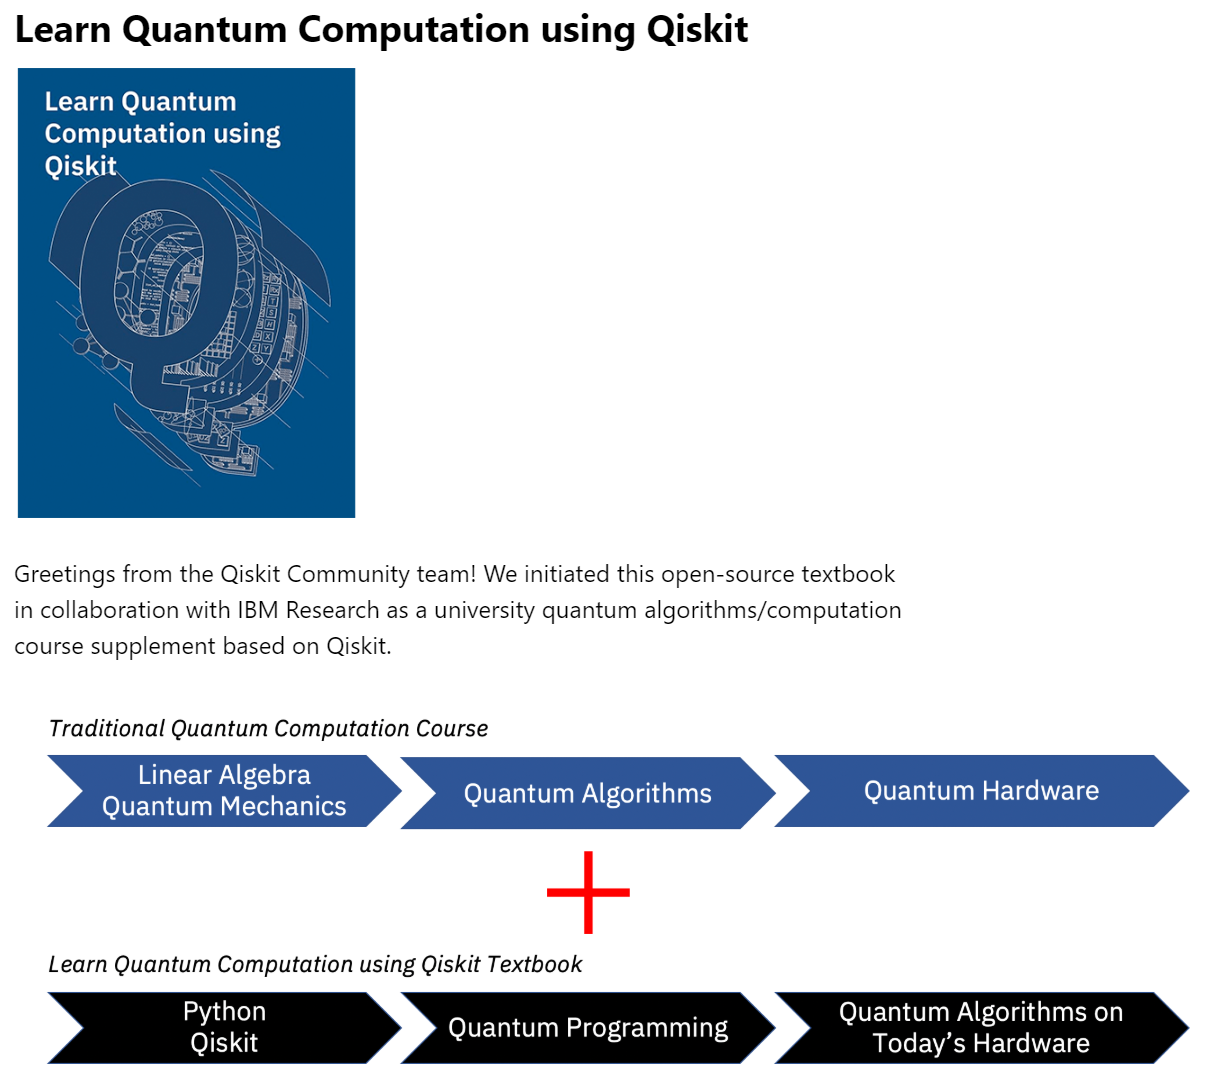
\includegraphics[width=\textwidth]{8.png}}
\caption{\url{https://qiskit.org/textbook/preface.html} (Quantum Computation using Qiskit)}
\label{fig}
\end{figure}
\newpage

Also, there are some other virtual quantum computing machines on other platforms. Such as MicrosoftQDK.

\begin{figure}[htbp]
\centerline{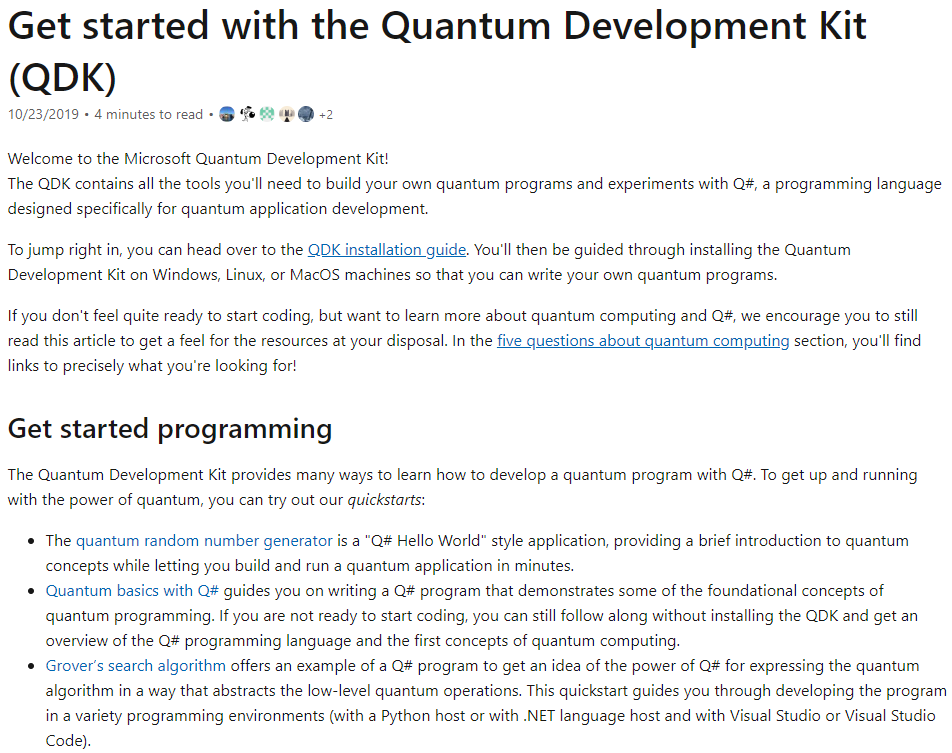
\includegraphics[width=\textwidth]{9.png}}
\caption{\url{https://docs.microsoft.com/en-us/quantum/welcome?view=qsharp-preview} (Microsoft QDK)}
\label{fig}
\end{figure}


As well as the basic operation of the virtual quantum computing machine, like how to install, how to create quantum circuit….

\url{https://quantum-computing.ibm.com/docs/qis-tut/} (Qiskit tutorials)
\newpage


\section{Code documentation}
Quantum programming is the process of assembling sequences of instructions, called quantum programs, that are capable of running on a quantum computer. 

In quantum computing, a qubit or quantum bit (sometimes qbit) is the basic unit of quantum information. So it determines quantum computer is different from normal computer, it can contain not only value 0 or value 1, but also contain some values which are in superposition state.

\subsection{Quantum Code}
Quantum programming is based on Q\# language, here is an example of Q# language from Microsoft.

\begin{figure}[htbp]
\centerline{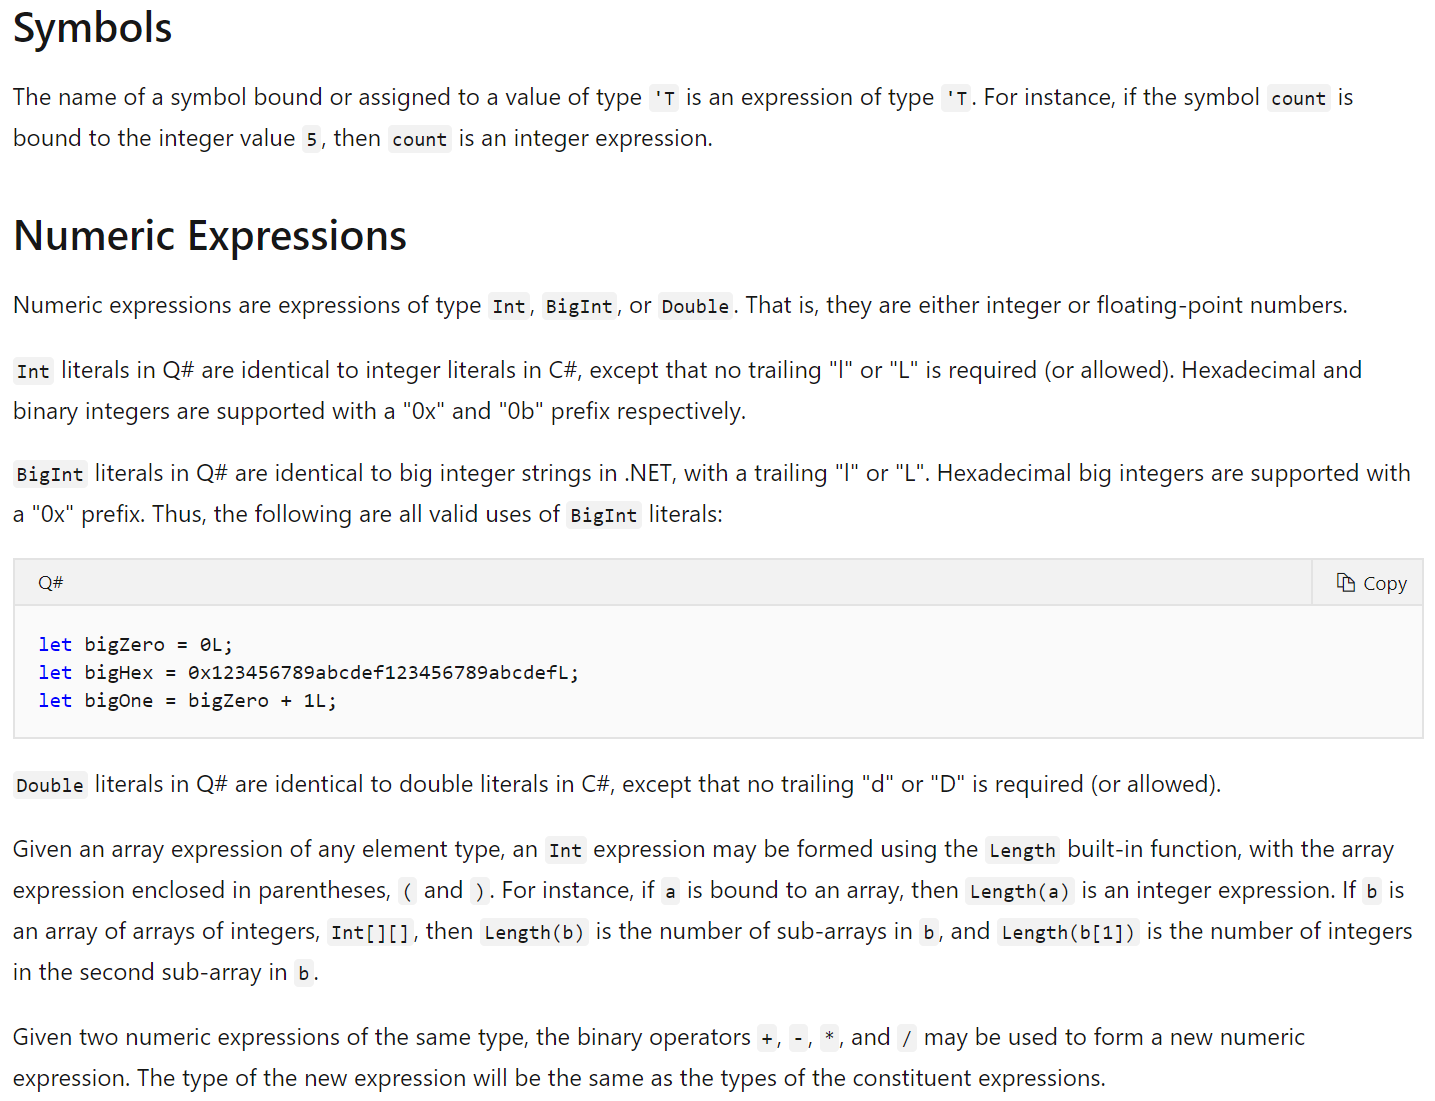
\includegraphics[width=\textwidth]{2.png}}
\caption{\url{https://docs.microsoft.com/en-us/quantum/language/expressions}}
\label{fig}
\end{figure}
\newpage

\begin{figure}[htbp]
\centerline{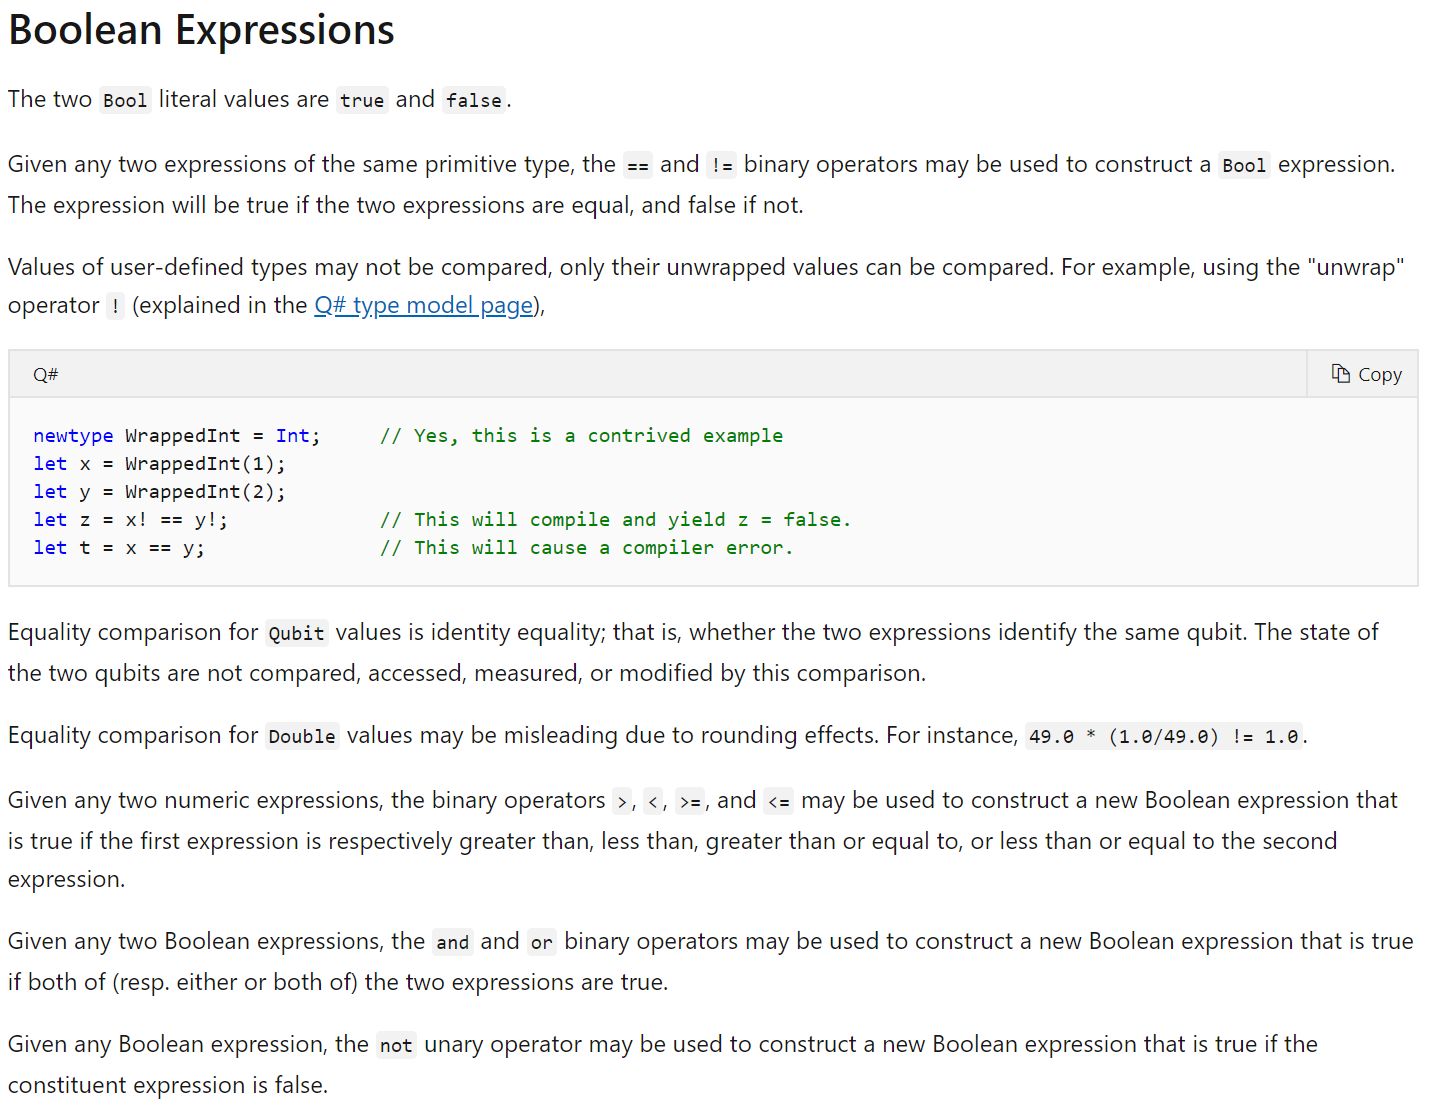
\includegraphics[width=\textwidth]{3.png}}
\caption{\url{https://docs.microsoft.com/en-us/quantum/language/expressions}}
\label{fig}
\end{figure}
\newpage

\subsection{Quantum Algorithm}
Just like modern computers, quantum computer also have to be based on quantum algorithm to solve problems. Here are some examples of quantum algorithm:


\begin{figure}[htbp]
\centerline{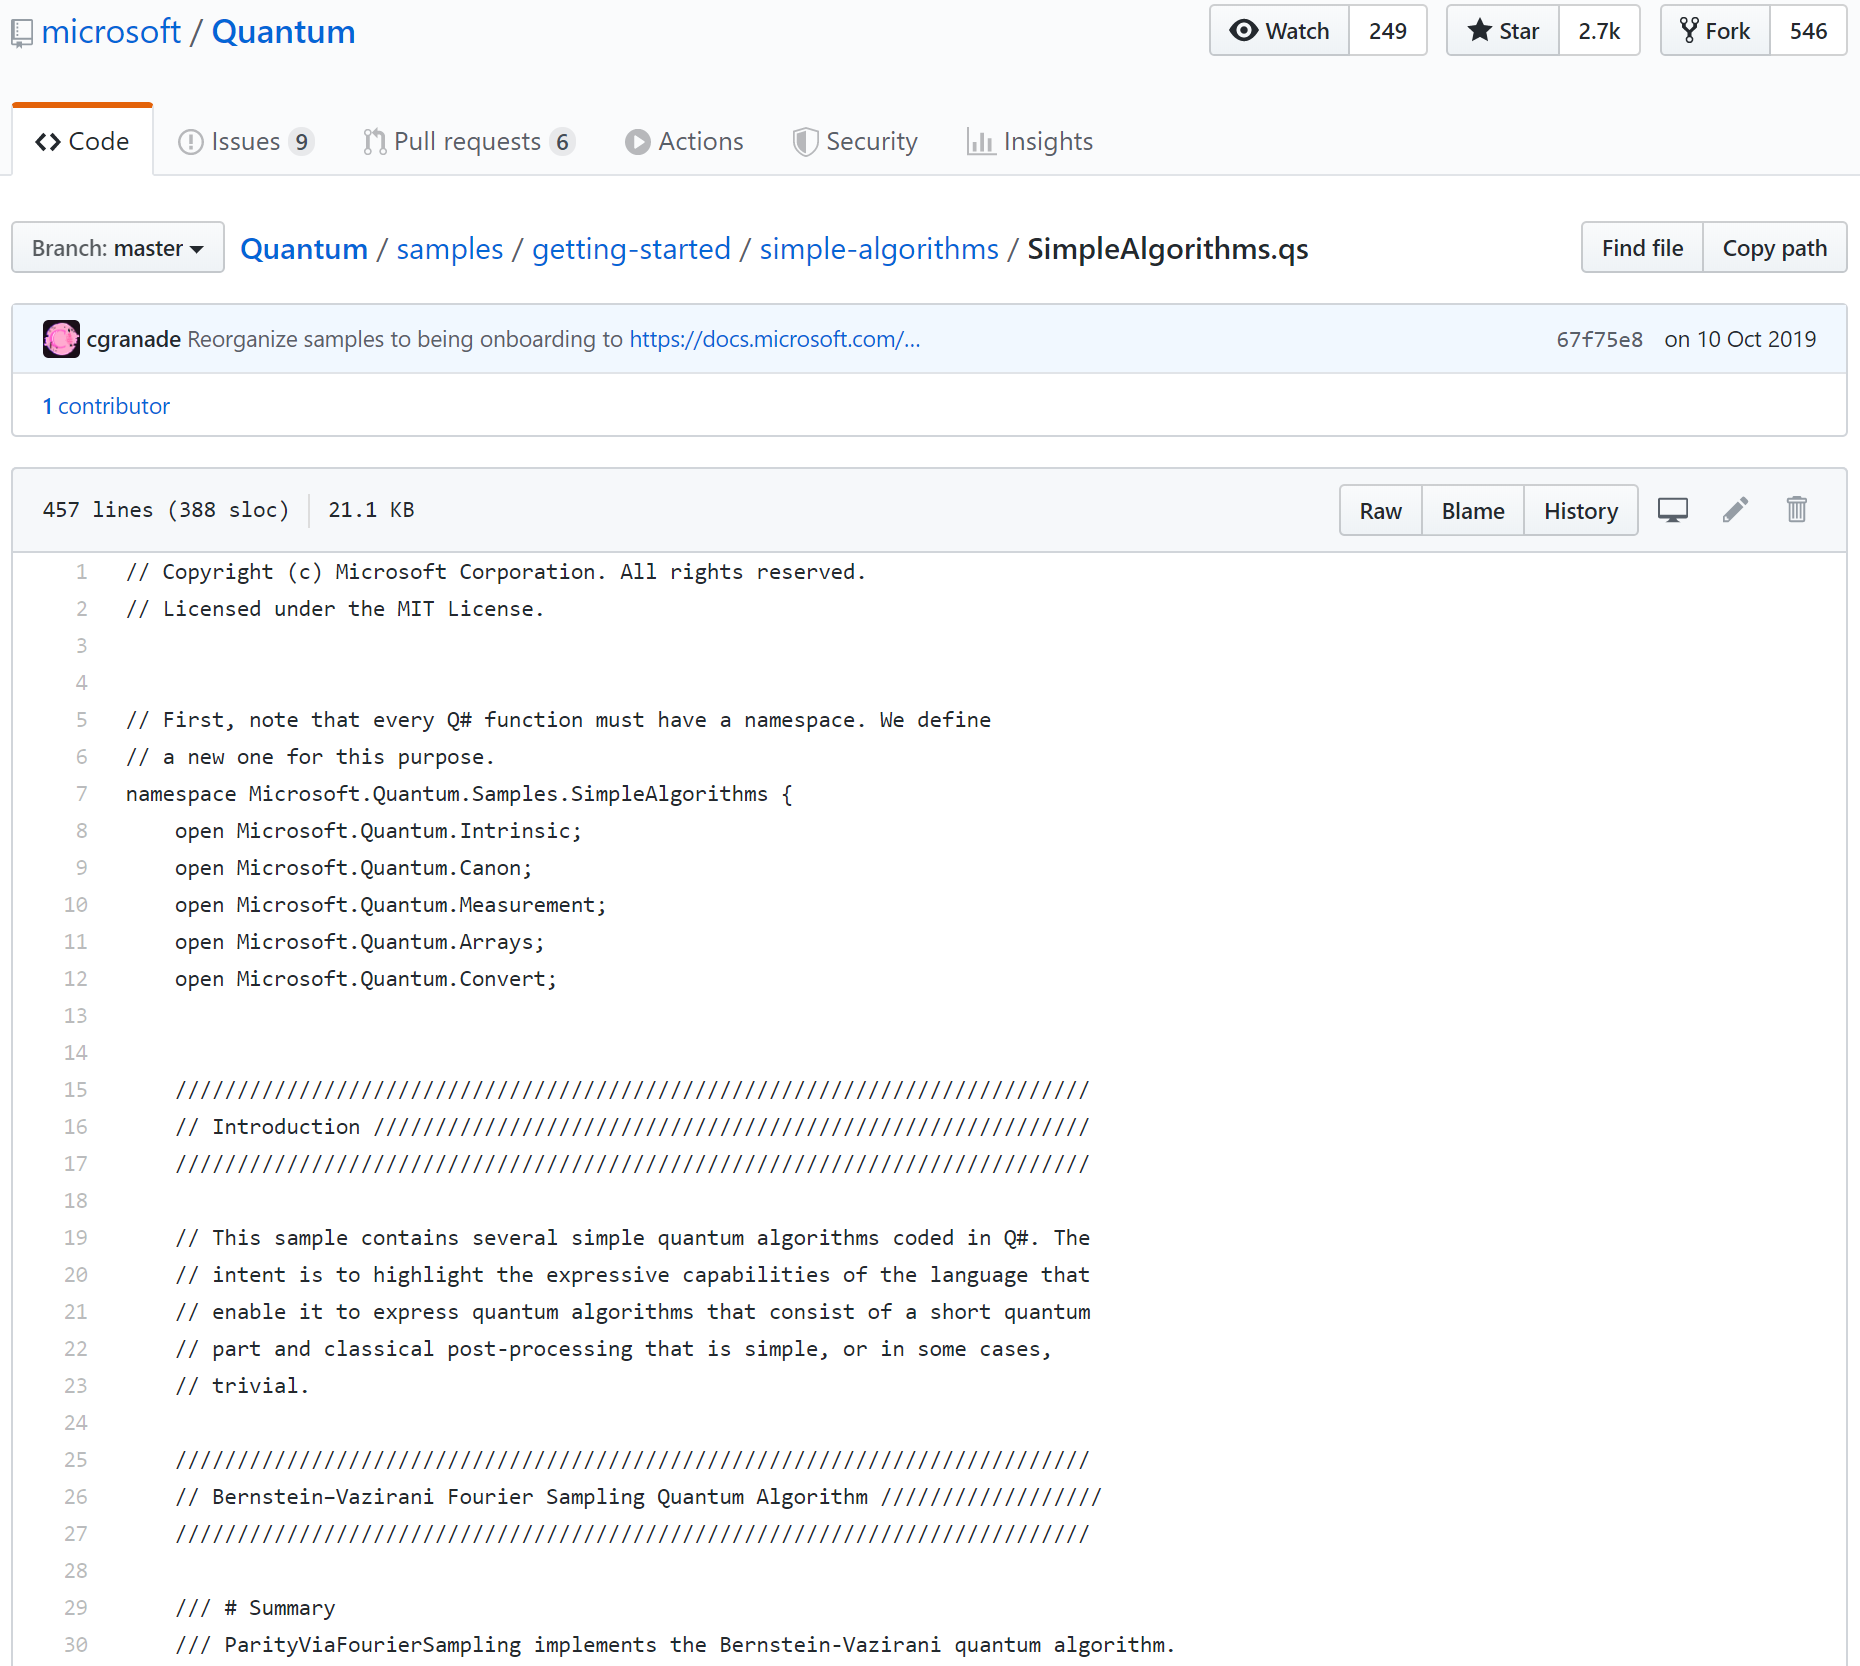
\includegraphics[width=\textwidth]{4.png}}
\caption{\url{https://github.com/microsoft/Quantum/blob/master/samples/getting-started/simple-algorithms/SimpleAlgorithms.qs }}
\label{fig}
\end{figure}


\newpage

And the classical quantum computing algorithm for integer factorization,Shor's algorithm that can factorize big integers in polynomial-time.

\begin{figure}[htbp]
\centerline{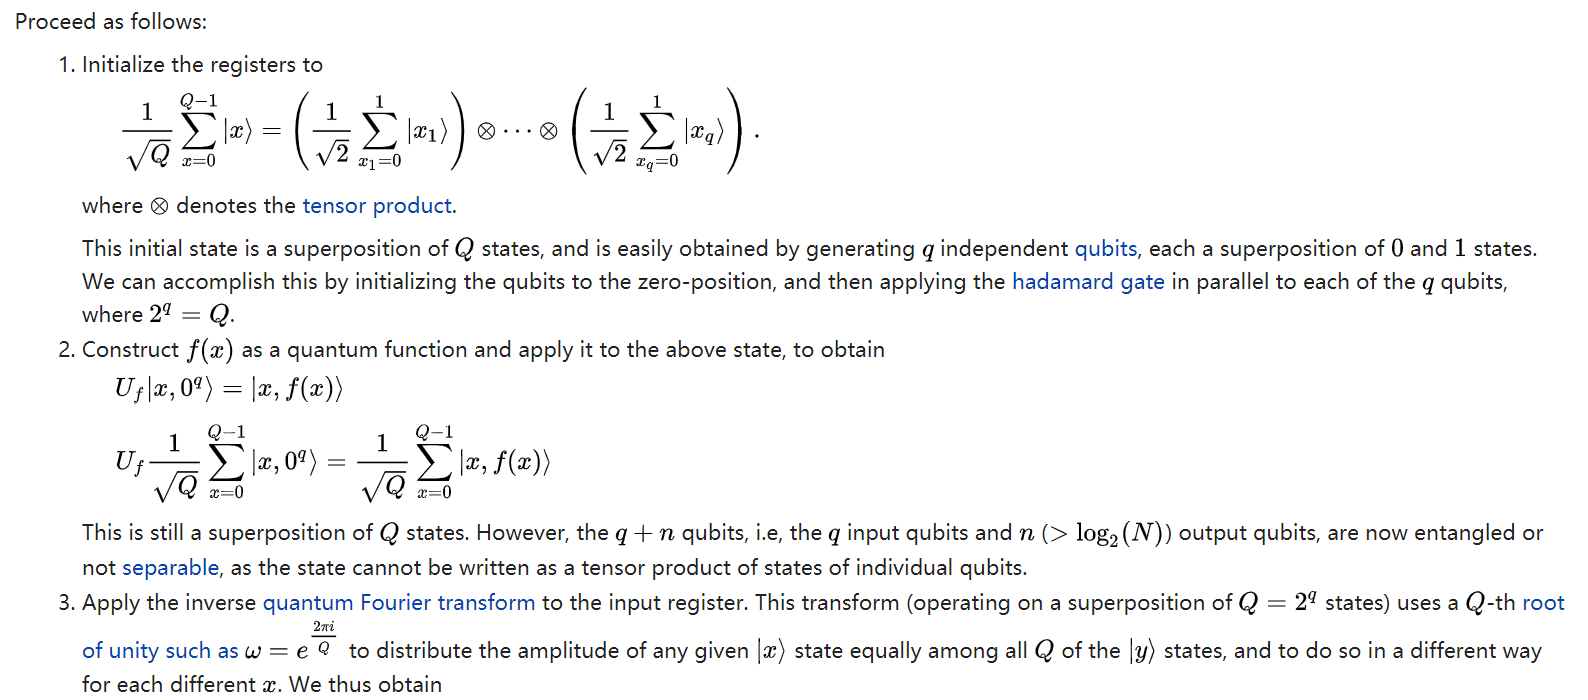
\includegraphics[width=\textwidth]{10.png}}
\caption{\url{https://en.wikipedia.org/wiki/Shor\%27s_algorithm}}
\label{fig}
\end{figure}
\newpage


\subsection{Quantum circuits}
In quantum computing there is a special programing which is quantum circuits.

\emph{A quantum circuit is a model for quantum computation in which a computation is a sequence of quantum gates, which are reversible transformations on a quantum mechanical analog of an n-bit register.}(\url{https://en.wikipedia.org/wiki/Quantum_circuit} )

Here is an example of quantum circuits based on IBM circuits composer experience:


\begin{figure}[htbp]
\centerline{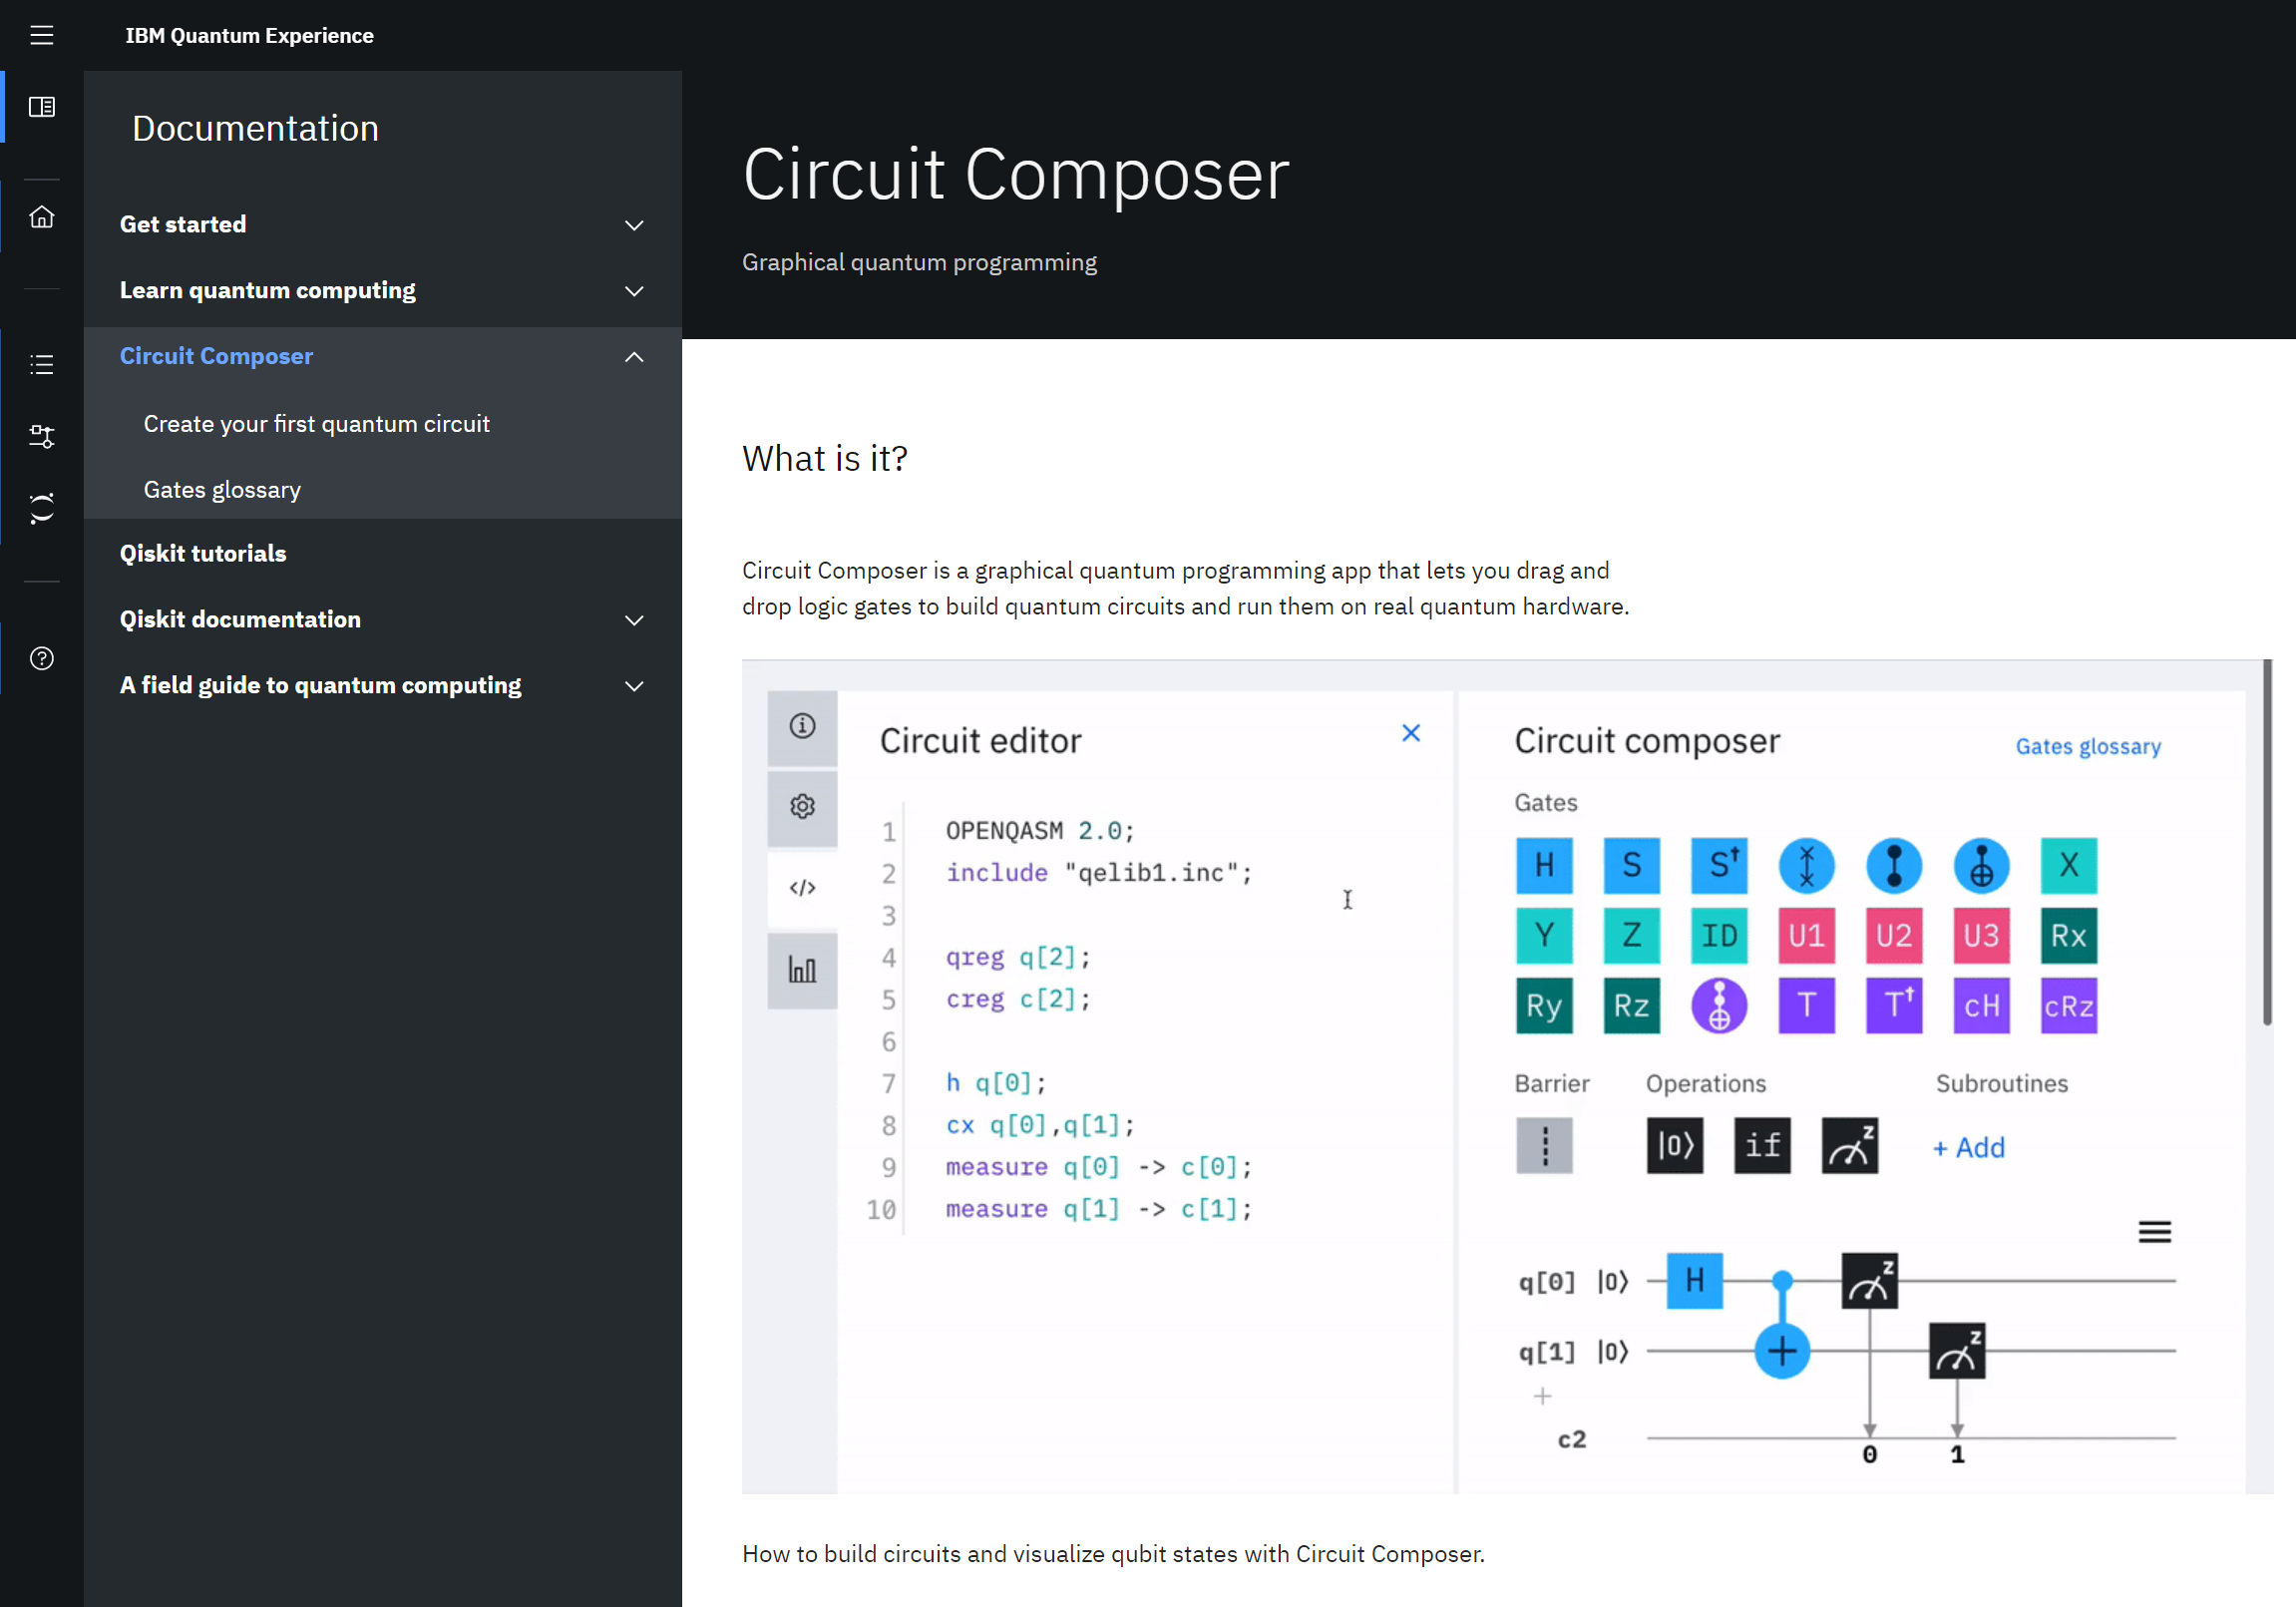
\includegraphics[width=\textwidth]{5.png}}
\caption{\url{https://quantum-computing.ibm.com/docs/circ-comp/}}
\label{fig}
\end{figure}


\newpage



\section{Community documentation}

Community documentation is an open source document. There are many forms and uses for the community documentation. One of the forms is Q&A. This form allows software developers to seek help from another software developer. Another form of community documentation is blog posts. This form is an open source documentation that is provided by the community to share their knowledge about the topic.

\subsection{Q&A}
As a new software developer who just started researching on quantum computing, reading the written documentation to understand the very basic terminology might be difficult. Thus, posting your question about quantum computing online can help you get a more understandable explanation to the problem you do not understand. Below is an example of Q&A form, explaining the basic of quantum computing.

\begin{figure}[htbp]
\centerline{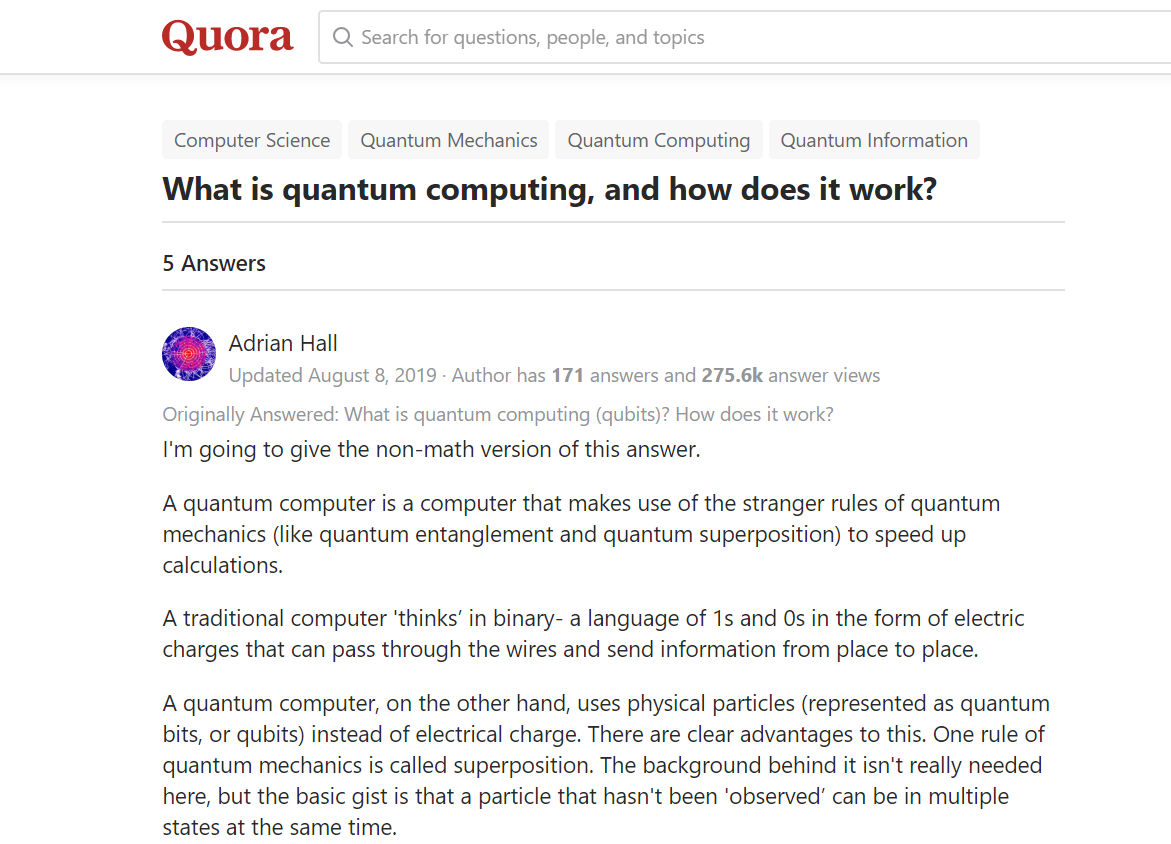
\includegraphics[width=\textwidth]{6.png}}
\caption{\url{https://www.quora.com/What-is-quantum-computing-and-how-does-it-work}}
\label{fig}
\end{figure}

Therefore, to get the general idea of quantum computing as a coprocessor and not just a stand alone computer. We can simply post our question and get the explanation from a Q&A form. Below is an example of an explanation received from a question about why quantum computing is not a stand alone computer.

\begin{figure}[htbp]
\centerline{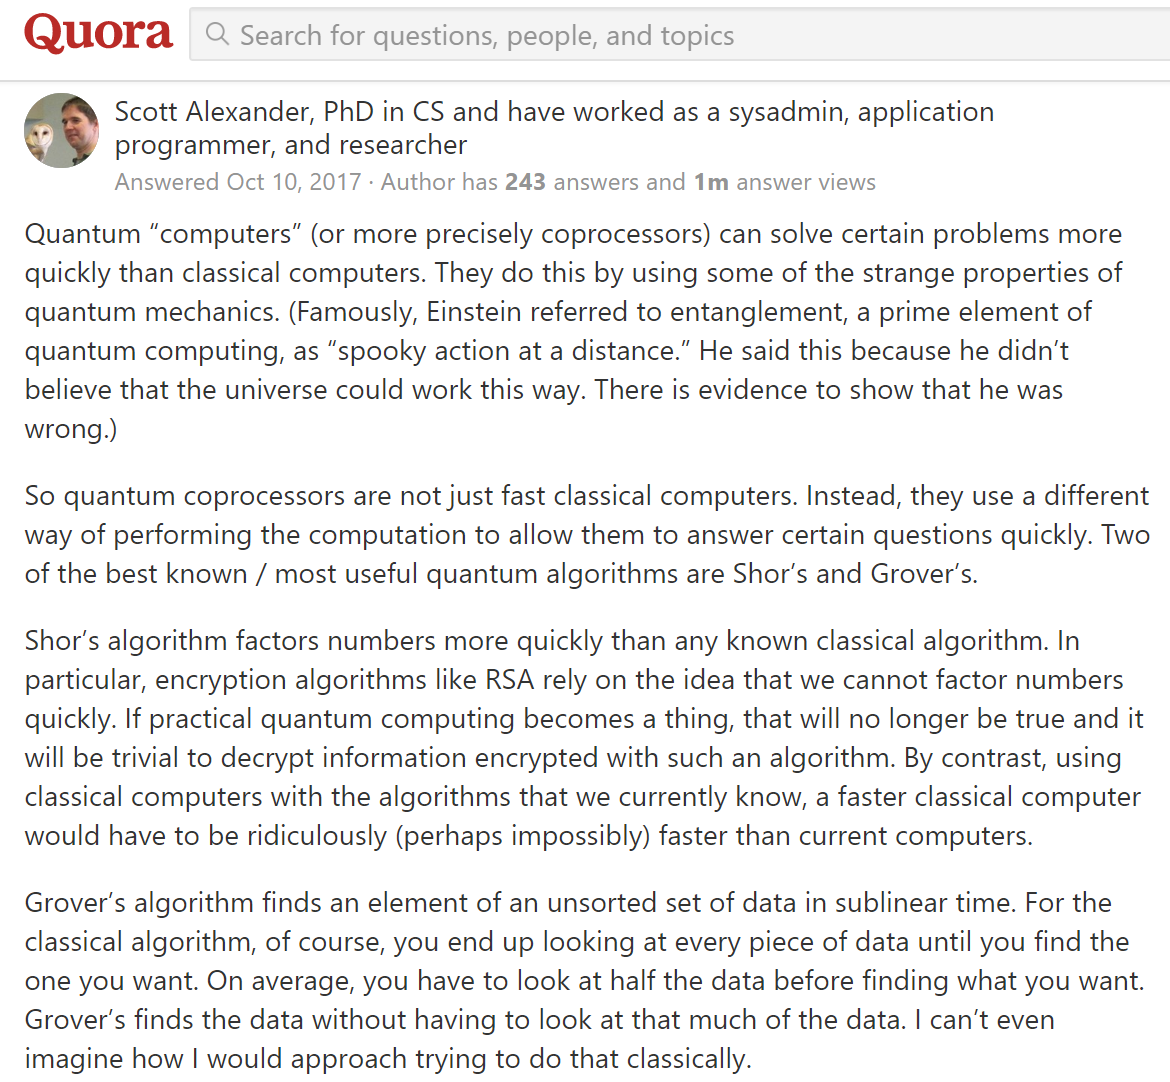
\includegraphics[width=\textwidth]{11.png}}
\caption{\url{https://www.quora.com/Is-a-quantum-computer-just-a-fast-computer}}
\label{fig}
\end{figure}
\newpage

\subsection{Blog post}
Since quantum computing is still in a developing stage, being able to get immediate update information can be crucial for software developers. Thus, with the help of a blog post from a company that works on quantum computing such as IBM. Software developers can now easily get the latest information about quantum computing. Below is a screenshot of IBM blog post page for quantum computing

\begin{figure}[htbp]
\centerline{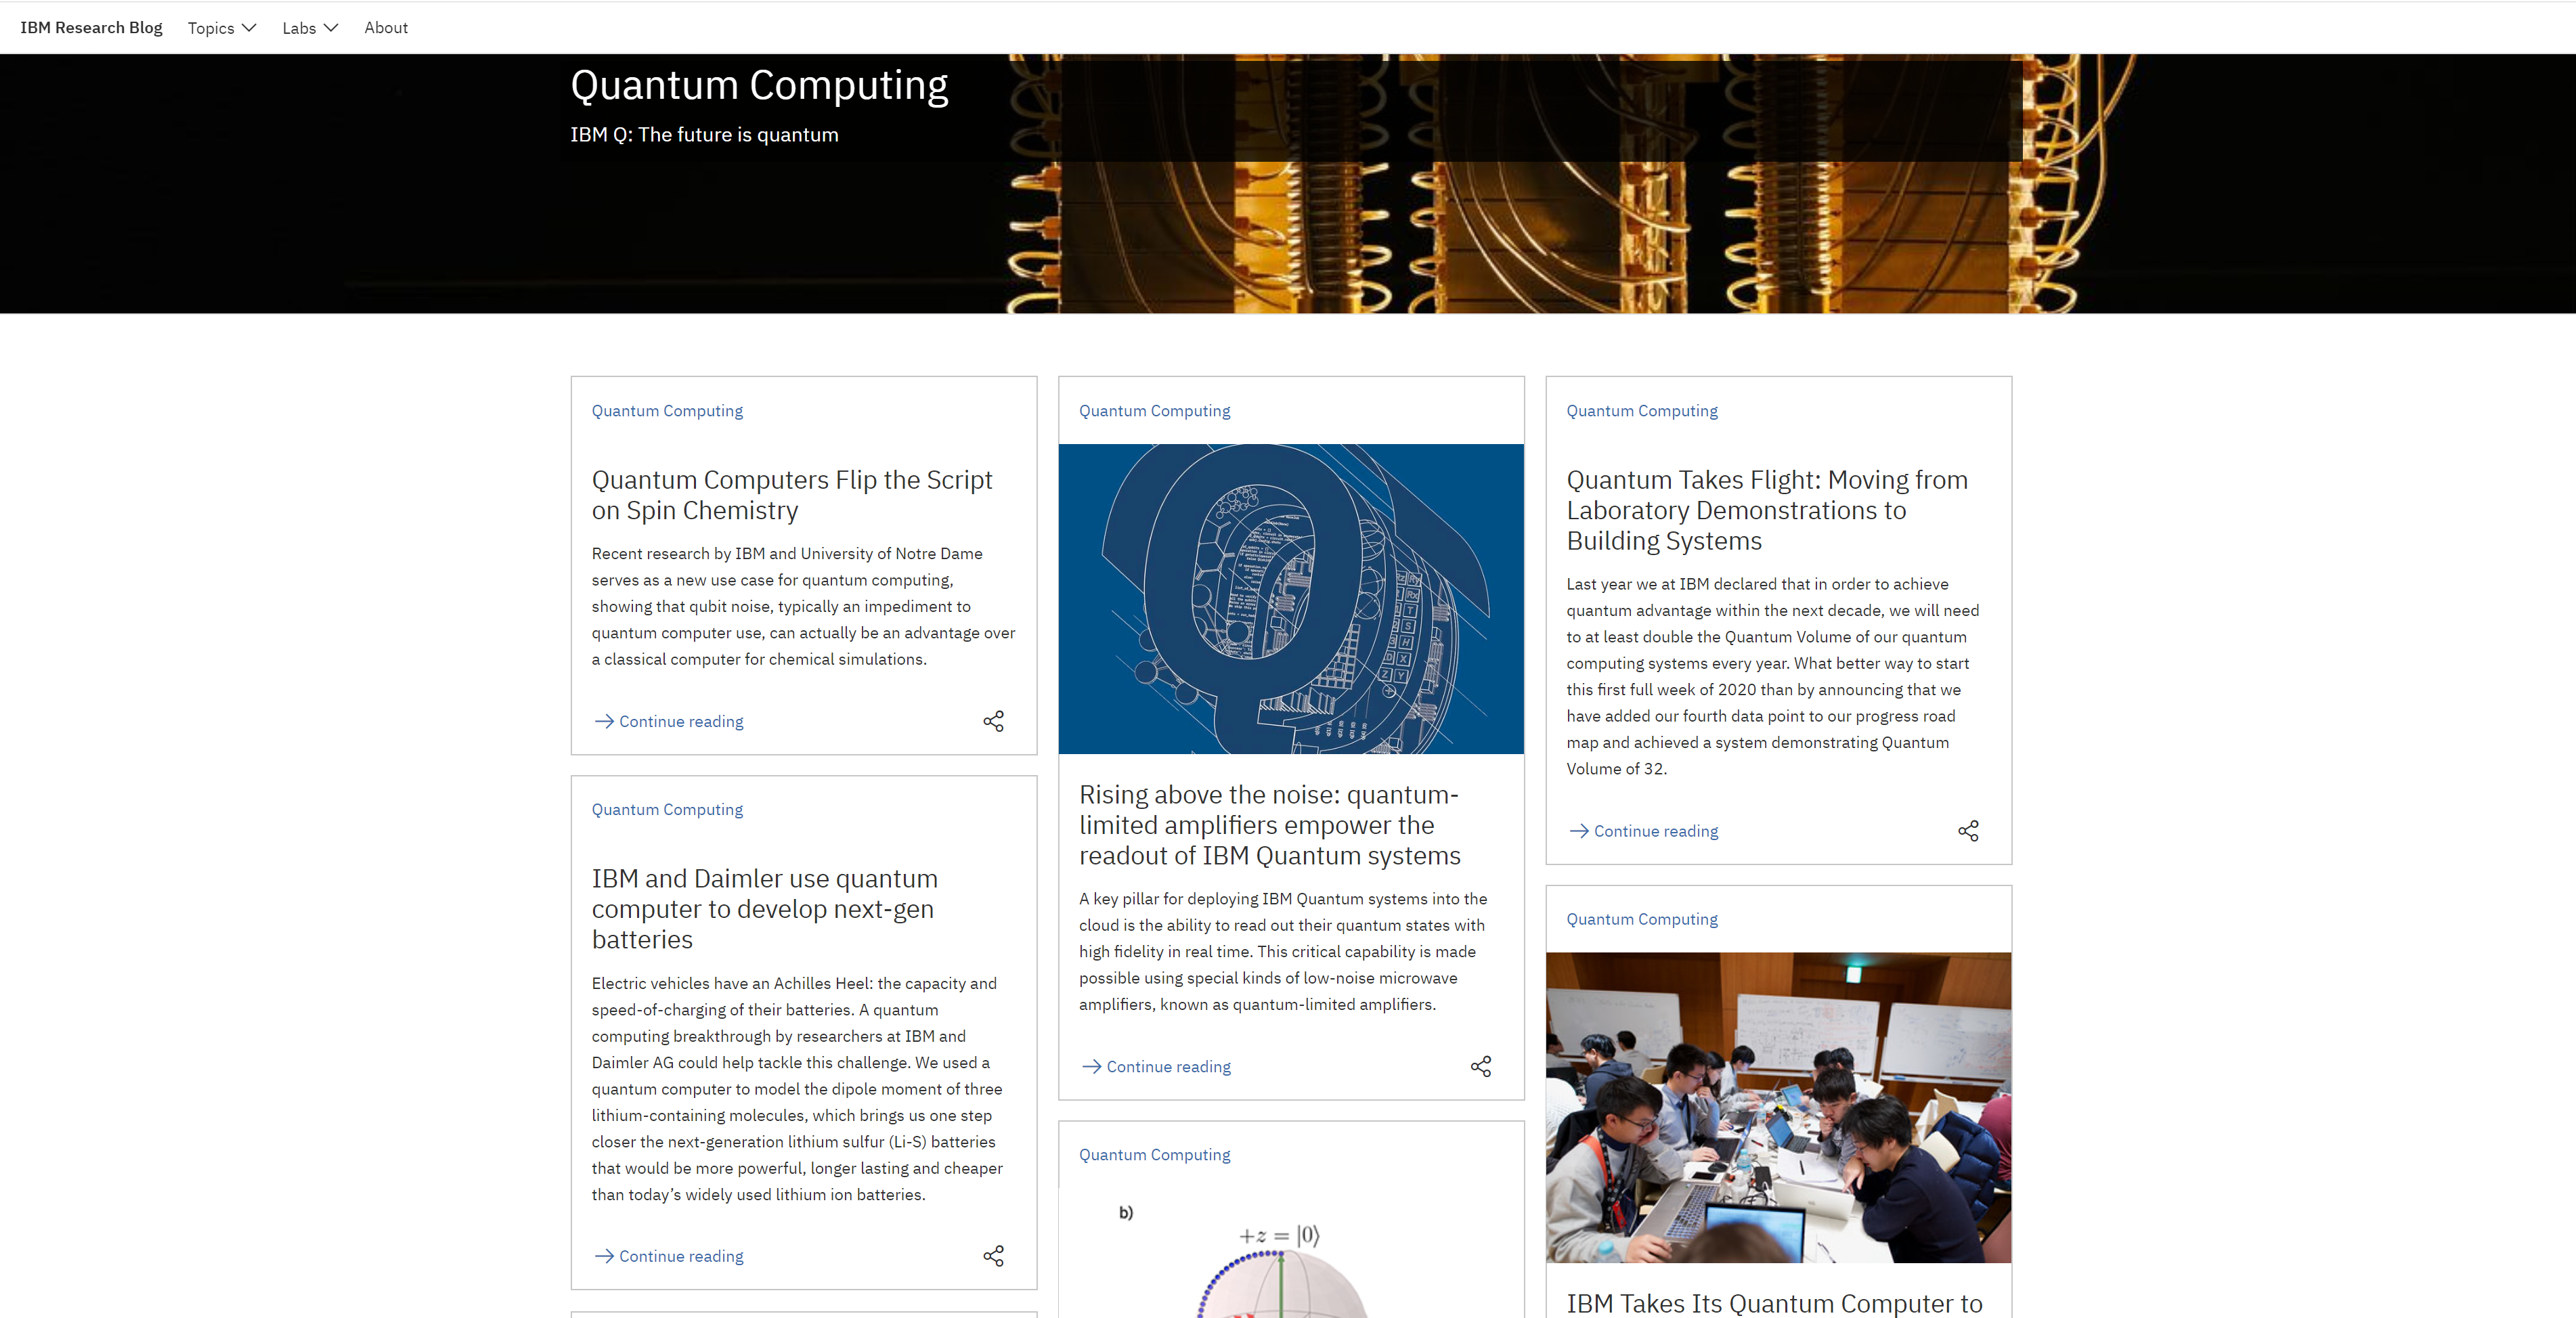
\includegraphics[width=\textwidth]{7.png}}
\caption{\url{https://www.ibm.com/blogs/research/category/quantcomp/}}
\label{fig}
\end{figure}
\newpage

\section{Conclusion}
In conclusion, there are quite a lot of advantages of quantum computer and quantum algorithms. Quantum computer uses qubits instead of bits compared with a normal computer. The normal bits can only store information as binary 0 and 1 states, while one qubit can store 2 states at the same time, which means if a quantum computer has 10 qubits, it can run 1024 states at the same time. That is equal to a normal computer use 1024 bits to run. If the quantum computer has large enough qubits like about 50, its efficiency is equal to thousands of normal computers run at the same time.

However, the quantum computer can not run without the quantum algorithm. Because like the normal computer, that we need to store the true and false value into register in order to perform calculation, qubits also need the quantum algorithm to run. For example the Shor’s algorithm, it can use qubits to solve the discrete logarithm problem and the integer factorization problem in polynomial time. 
Also,  the qubits use photons or some other particles as a physical medium and they need to have a very strict environment to keep their excited state. 

Quantum computers can not run by itself. A reasonable quantum computer, should be implemented with a suitable quantum algorithm, and an environment that  keeps photons or particles in excited state and so on. Therefore, it can be thought of as a co-processor.



\end{document}
